
\hypertarget{menu_help}{}
\section{Help}
\index{help menu}
\index{user guide}
\index{ini file}
\index{recognized words}
\index{about}
\index{User list}
\index{Discussion group}

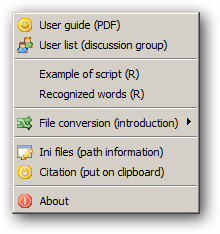
\includegraphics[scale=0.50]{./res/menu_help.png}\\

\begin{scriptsize}\begin{tabularx}{\textwidth}{>{\hsize=0.3\hsize}X>{\hsize=0.7\hsize}X}\\
    \hline
    \textbf{Option} & \textbf{Description} \\
    \hline
    User guide (PDF) & Opens the User guide with the PDF viewer default \\
    User list (discussion group) & Opens URL \htmladdnormallink{Tinn-R Editor - GUI for R Language and Environment user list}{http://groups.google.com/forum/?fromgroups\#!forum/tinn-r} \\
    Recognized words (R) & Opens the file \textit{Tinn-R\_recognized words.r} \\
    Example of script (R) & Opens the file \textit{Tinn-r\_example of script.r} \\
    File conversion (introduction) & \textit{\htmladdnormallink{See options ...}{\#menu\_help\_main\_fileconversion}} \\
    Ini files (path information) & Displays a single dialog with the path information of ini files for Tinn-R \\
    Citation (put on clipboard) & Places a text containing the Tinn-R citation in the clipboard \\
    About & Opens the dialog About \\
    \hline
  \end{tabularx}\end{scriptsize}


\hypertarget{menu_help_main_fileconversion}{}
\subsubsection{File conversion (introduction):}\\
\index{help menu!main file conversion}

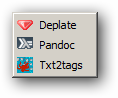
\includegraphics[scale=0.50]{./res/menu_help_conversion.png}\\

\begin{scriptsize}\begin{tabularx}{\textwidth}{>{\hsize=0.3\hsize}X>{\hsize=0.7\hsize}X}\\
    \hline
    \textbf{Option} & \textbf{Description} \\
    \hline
    Deplate & Opens the file \textit{deplate\_intro.t2t} \\
    Pandoc & Opens the file \textit{pandoc.markdown} \\
    Txt2tags & Opens the file \textit{txt2tags\_intro.t2t} \\
    \hline
  \end{tabularx}\end{scriptsize}
